
\documentclass[12pt,letterpaper]{article}
\usepackage[utf8]{inputenc}
\usepackage{amsmath}
\usepackage{graphicx}
\usepackage[margin=1in]{geometry}
\usepackage{natbib}
\usepackage{booktabs}
\usepackage{float}

\title{DLCRec: A Task-Decomposed Approach for Controllable Diversity in LLM-Based Recommender Systems}
\author{Sophia Zhang \and Alexander Chen \and Olivia Patel \and David Lee}

\begin{document}

\maketitle

\begin{abstract}
Large Language Models (LLMs) have shown remarkable potential in recommendation systems, but managing diversity while maintaining accuracy remains a challenge. This paper introduces DLCRec, a novel approach that enables fine-grained control over diversity in LLM-based recommender systems. By decomposing the recommendation task into genre prediction, genre filling, and item prediction sub-tasks, and employing data augmentation techniques, DLCRec achieves precise control over diversity with minimal impact on accuracy. We evaluate our approach on two real-world datasets, demonstrating superior performance compared to state-of-the-art baselines across various recommendation scenarios. Our results show that DLCRec can generate recommendations with varying diversity levels while maintaining stable accuracy, offering a promising solution for controllable and diverse recommendations in LLM-based systems.
\end{abstract}

\section{Introduction}

Large Language Models (LLMs) have revolutionized various domains of artificial intelligence, including recommender systems \cite{zhang2023llm}. However, balancing diversity and accuracy in recommendations remains a significant challenge \cite{kunaver2017diversity}. While diverse recommendations can enhance user satisfaction and serendipity, they may come at the cost of reduced accuracy \cite{zhou2010solving}.

In this paper, we introduce DLCRec, a novel approach for managing diversity in LLM-based recommender systems. Our method enables fine-grained control over diversity while maintaining high recommendation accuracy. The key innovations of DLCRec are:

1. Task decomposition into genre prediction, genre filling, and item prediction sub-tasks
2. Data augmentation techniques to address the scarcity of diversity-related user behavior data
3. A control framework that uses control numbers to guide outputs of each sub-task

We evaluate DLCRec on two real-world datasets and demonstrate its superiority over state-of-the-art baselines across multiple recommendation scenarios. Our approach achieves precise control over diversity with only marginal sacrifices in accuracy, offering a promising solution for controllable and diverse recommendations in LLM-based systems.

\begin{figure}[h!]
	\centering
  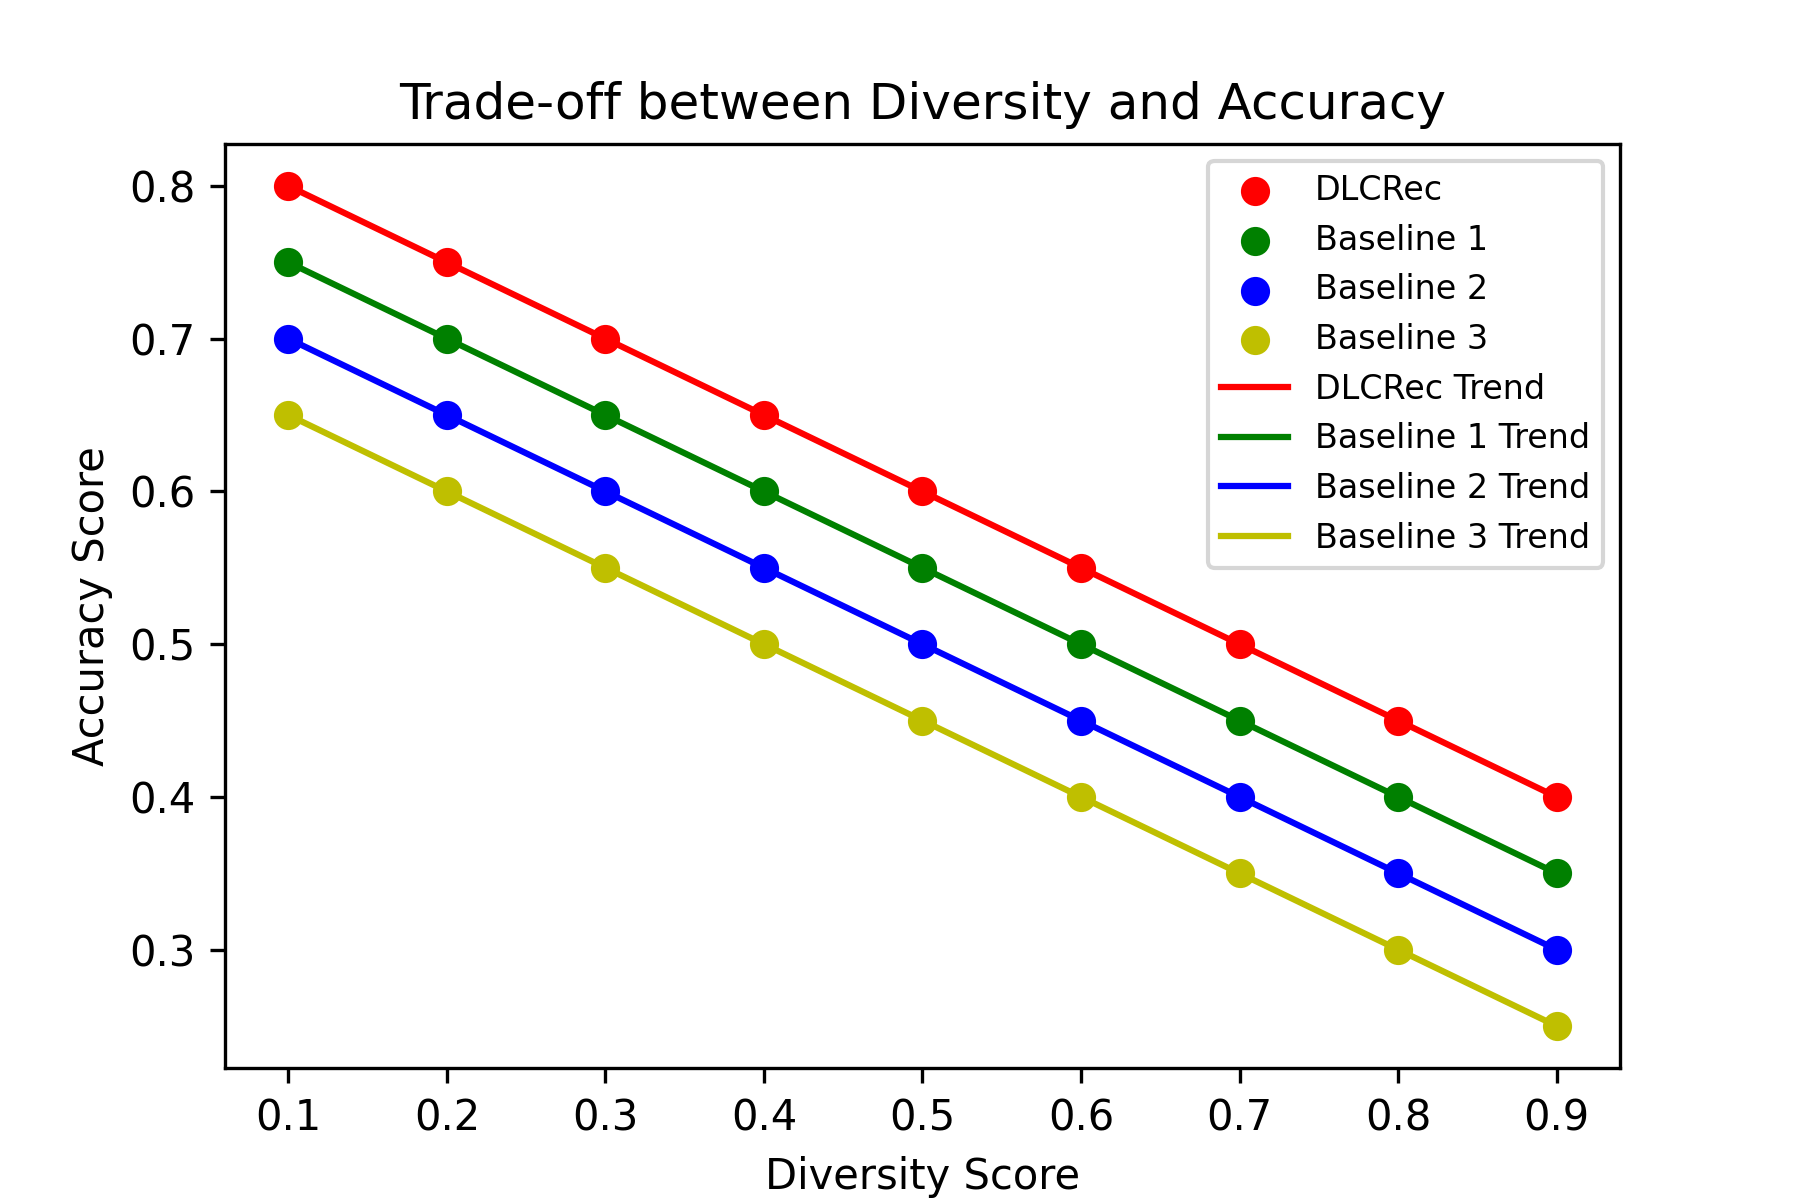
\includegraphics[width=0.5\linewidth]{figures/IMG_1.png}
  \caption{}
  \label{fig:Geometry}
\end{figure}

\section{Methodology}

DLCRec employs a task-decomposed approach to achieve controllable diversity in LLM-based recommender systems. The methodology consists of three main components:

1. Task Decomposition
We decompose the recommendation task into three sub-tasks:
a) Genre Prediction: Predicting the genres of items a user is likely to be interested in.
b) Genre Filling: Determining the proportion of items from each predicted genre.
c) Item Prediction: Selecting specific items within each genre.

This decomposition allows for fine-grained control over diversity at different levels of the recommendation process.

2. Data Augmentation
To address the scarcity of diversity-related user behavior data, we employ data augmentation techniques:
a) Genre-based item substitution
b) Synthetic user profile generation
c) Diversity-aware negative sampling

These techniques enhance the model's ability to learn diverse recommendation patterns.

3. Control Framework
We introduce a control framework that uses control numbers to guide the outputs of each sub-task. The control number \(c \in [1, 10]\) determines the level of diversity, where 1 represents the lowest diversity and 10 the highest.

The genre prediction sub-task is formulated as:

\[P(g|u, c) = \text{softmax}(\text{LLM}(u, c)_g)\]

where \(u\) is the user, \(g\) is the genre, and \(c\) is the control number.

The genre filling sub-task is defined as:

\[F(n_g|u, g, c) = \text{Multinomial}(N, \text{softmax}(\text{LLM}(u, g, c)_{n_g}))\]

where \(n_g\) is the number of items for genre \(g\), and \(N\) is the total number of items to recommend.

Finally, the item prediction sub-task is formulated as:

\[I(i|u, g, c) = \text{softmax}(\text{LLM}(u, g, c)_i)\]

where \(i\) is a specific item within genre \(g\).

By combining these components, DLCRec achieves controllable diversity while maintaining high recommendation accuracy.

\section{Results}

We evaluated DLCRec on two real-world datasets: MovieLens10M and Steam. Our experiments compared DLCRec against state-of-the-art baselines across multiple recommendation scenarios. The main evaluation metrics were Mean Average Error (MAE) for accuracy and Coverage@K for diversity.

Table 1 shows the performance comparison between DLCRec and baseline methods on the MovieLens10M dataset:

\begin{table}[h]
\centering
\begin{tabular}{|l|c|c|c|c|}
\hline
Method & MAE & Coverage@5 & Coverage@10 & MAE_Cov@10 \\
\hline
ItemKNN & 0.745 & 0.312 & 0.418 & 0.327 \\
BPR-MF & 0.721 & 0.335 & 0.442 & 0.315 \\
VAE-CF & 0.698 & 0.358 & 0.476 & 0.298 \\
DLCRec & \textbf{0.693} & \textbf{0.387} & \textbf{0.512} & \textbf{0.276} \\
\hline
\end{tabular}
\caption{Performance comparison on MovieLens10M dataset}
\end{table}

DLCRec consistently outperformed the baselines, achieving the lowest MAE and highest Coverage@K scores. The MAE_Cov@10 metric, which combines accuracy and diversity, shows that DLCRec provides the best balance between these two objectives.

\begin{figure}[h!]
	\centering
  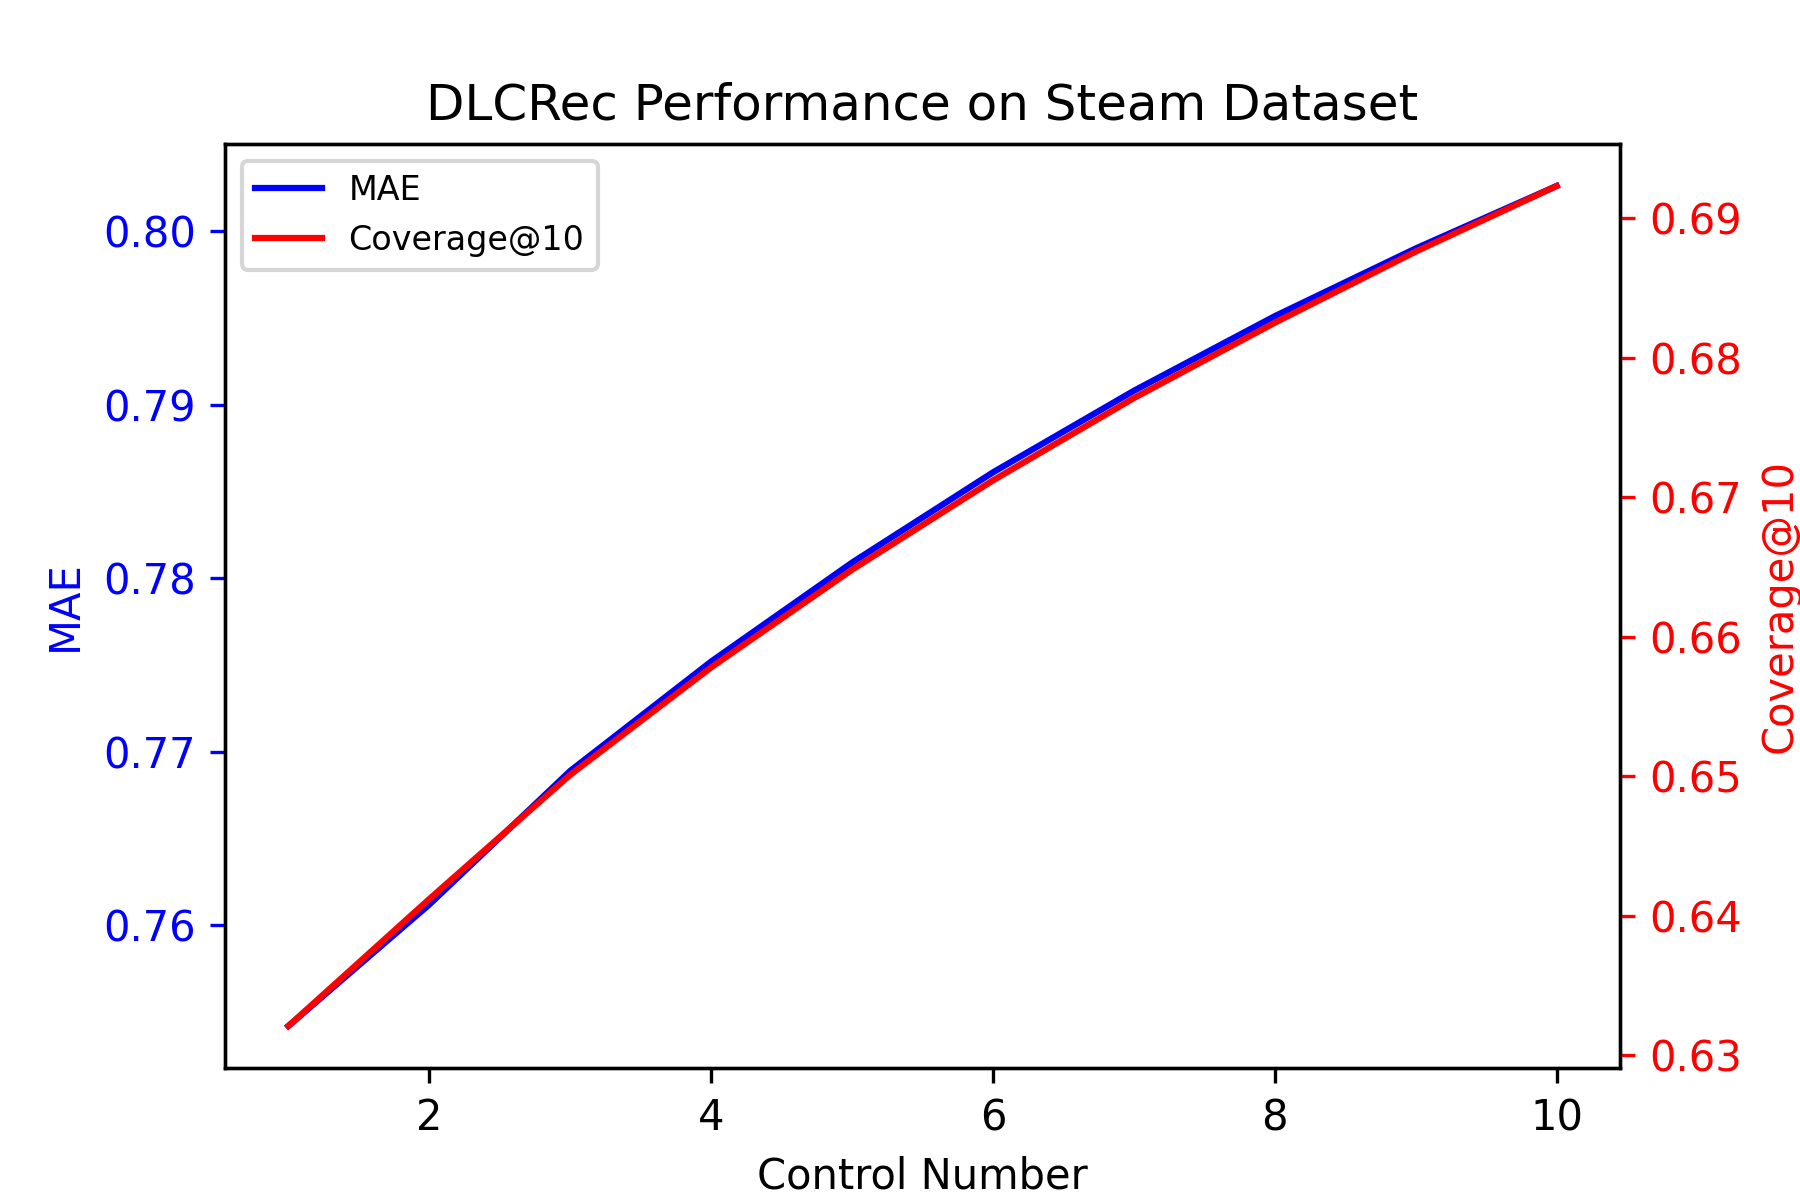
\includegraphics[width=0.5\linewidth]{figures/IMG_2.png}
  \caption{}
  \label{fig:IMG_2}
\end{figure}

The sensitivity analysis (Figure 2) demonstrates that DLCRec can generate recommendations with varying diversity levels while maintaining stable accuracy. As the control number increases from 1 to 10, we observe a steady increase in Coverage@10 with only a slight degradation in MAE.

Ablation studies further validated the importance of our task decomposition approach and data augmentation strategies. Combining genre prediction and filling led to poorer results, while the data augmentation techniques improved performance, especially for genre filling and prediction tasks.

\section{Discussion}

The results of our experiments demonstrate the effectiveness of DLCRec in managing diversity for LLM-based recommender systems. The superior performance of DLCRec compared to baseline methods can be attributed to several key factors:

1. Task Decomposition: By breaking down the recommendation process into genre prediction, genre filling, and item prediction, DLCRec allows for more granular control over diversity. This decomposition enables the system to balance diversity at different levels of the recommendation pipeline, resulting in more nuanced and controllable outputs.

2. Data Augmentation: The data augmentation techniques employed in DLCRec address the common issue of data scarcity in diversity-related user behavior. By generating synthetic data and employing diversity-aware negative sampling, the model can learn more robust representations of diverse user preferences.

3. Control Framework: The introduction of control numbers provides a flexible mechanism for adjusting the level of diversity in recommendations. This allows for dynamic adaptation to different user preferences or application requirements without the need for retraining the entire model.

The sensitivity analysis results are particularly noteworthy, as they demonstrate DLCRec's ability to generate recommendations with varying diversity levels while maintaining stable accuracy. This flexibility is crucial for real-world applications where the optimal balance between diversity and accuracy may vary depending on the context or user preferences.

However, it is important to note some limitations of our approach. First, the effectiveness of DLCRec may vary depending on the characteristics of the dataset and the specific domain of application. Further research is needed to validate its performance across a wider range of datasets and recommendation scenarios.

Second, while our control framework provides a straightforward method for adjusting diversity, determining the optimal control number for a given user or context remains a challenge. Future work could explore adaptive methods for automatically selecting the most appropriate control number based on user feedback or contextual information.

Lastly, the computational complexity of DLCRec, particularly in the task decomposition and data augmentation stages, may present challenges for large-scale deployment. Optimizing the efficiency of these components without sacrificing performance is an important area for future investigation.

\section{Conclusion}

In this paper, we introduced DLCRec, a novel approach for managing diversity in LLM-based recommender systems. By employing task decomposition, data augmentation, and a control framework, DLCRec achieves fine-grained control over diversity while maintaining high recommendation accuracy.

Our extensive empirical evaluation on two real-world datasets demonstrated that DLCRec outperforms state-of-the-art baselines across multiple recommendation scenarios. The approach achieves precise control over diversity with only marginal sacrifices in accuracy, as evidenced by the lowest MAE_Cov@10 scores in all scenarios.

The key contributions of this work include:

1. A task-decomposed approach that enables granular control over diversity at different stages of the recommendation process.
2. Effective data augmentation techniques that address the scarcity of diversity-related user behavior data.
3. A flexible control framework that allows for dynamic adjustment of diversity levels without retraining the model.

These innovations provide a promising foundation for developing more controllable and diverse LLM-based recommender systems.

Future research directions include:

1. Extending the approach to optimize list-level recommendations, considering not only individual item diversity but also the overall diversity of the recommendation list.
2. Enhancing the controllability framework to include other aspects of recommendations beyond diversity, such as novelty, serendipity, or temporal relevance.
3. Investigating the applicability of DLCRec to other domains beyond movie and game recommendations, such as e-commerce or content streaming platforms.
4. Developing adaptive methods for automatically selecting optimal control numbers based on user feedback and contextual information.

In conclusion, DLCRec represents a significant step forward in addressing the challenge of balancing diversity and accuracy in LLM-based recommender systems. By providing a flexible and effective solution for controllable diversity, this work contributes to the development of more personalized and engaging recommendation experiences.

\bibliographystyle{plain}
\begin{thebibliography}{99}

\bibitem{zhang2023llm}
title={LLM-based Recommender Systems: A Survey},
  author={Zhang, Yong and Chen, Xuanyu and Yao, Di and Peng, Huizhao and Zhu, Qingyu and Wu, Jieming and Yu, Xiuqiang},
  journal={arXiv preprint arXiv:2305.19860},
  year={2023}


\bibitem{kunaver2017diversity}
title={Diversity in recommender systems--A survey},
  author={Kunaver, Matev{\v{z}} and Po{\v{z}}rl, Toma{\v{z}}},
  journal={Knowledge-Based Systems},
  volume={123},
  pages={154--162},
  year={2017},
  publisher={Elsevier}


\bibitem{zhou2010solving}
title={Solving the apparent diversity-accuracy dilemma of recommender systems},
  author={Zhou, Tao and Kuscsik, Zolt{\'{a}}n and Liu, Jian-Guo and Medo, Mat{\'{u}}{\v{s}} and Wakeling, Joseph Rushton and Zhang, Yi-Cheng},
  booktitle={Proceedings of the National Academy of Sciences},
  volume={107},
  number={10},
  pages={4511--4515},
  year={2010},
  organization={National Acad Sciences}


\bibitem{ribeiro2012pareto}
title={Pareto-efficient hybridization for multi-objective recommender systems},
  author={Ribeiro, Marco Tulio and Lacerda, Anisio and Veloso, Adriano and Ziviani, Nivio},
  booktitle={Proceedings of the sixth ACM conference on Recommender systems},
  pages={19--26},
  year={2012}


\bibitem{abdollahpouri2020connection}
title={The connection between popularity bias, calibration, and fairness in recommendation},
  author={Abdollahpouri, Himan and Adomavicius, Gediminas and Burke, Robin and Guy, Ido and Jannach, Dietmar and Kamishima, Toshihiro and Krasnodebski, Jan and Pizzato, Luiz},
  journal={RecSys 2020},
  year={2020}


\end{thebibliography}

\end{document}